\chapter{Setting up the Workspace for Java Projects}

ETrice generates code out of ROOM models. The code generator and the generated code relies on a runtime framework and on some ready to use model parts. This parts provide services like:

\begin{itemize}
\item messaging
\item logging
\item timing
\end{itemize}

Additionally some tutorial models will be provided to make it easy to start with eTrice. All this parts must be available in our workspace before you can start working. After installation of eclipse (juno) and the eTrice plug in, your workspace should look like this:  

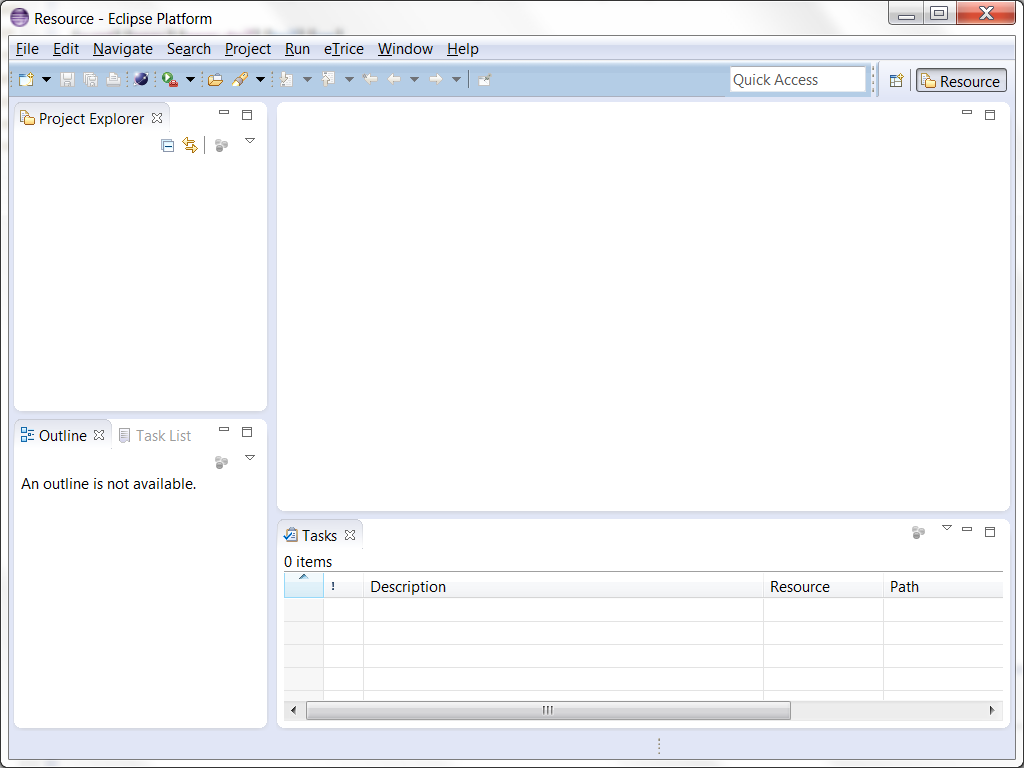
\includegraphics[width=\linewidth]{images/013-SetupWorkspace01.png}
% !images/013-SetupWorkspace01.png!

Just the \textit{eTrice} menu item is visible from the eTrice tool.
From the \textit{File} menu select \textbf{File->New->Project}

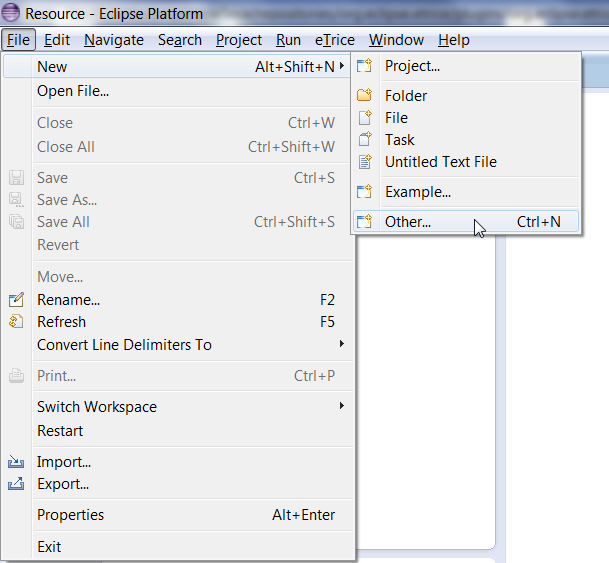
\includegraphics[width=\linewidth]{images/013-SetupWorkspace02.png}
% !images/013-SetupWorkspace02.png!

Open the \textit{eTrice} tab and select \textit{eTrice Java Runtime}

Press \textit{Next} and \textit{Finish} to install the Runtime into your workspace.

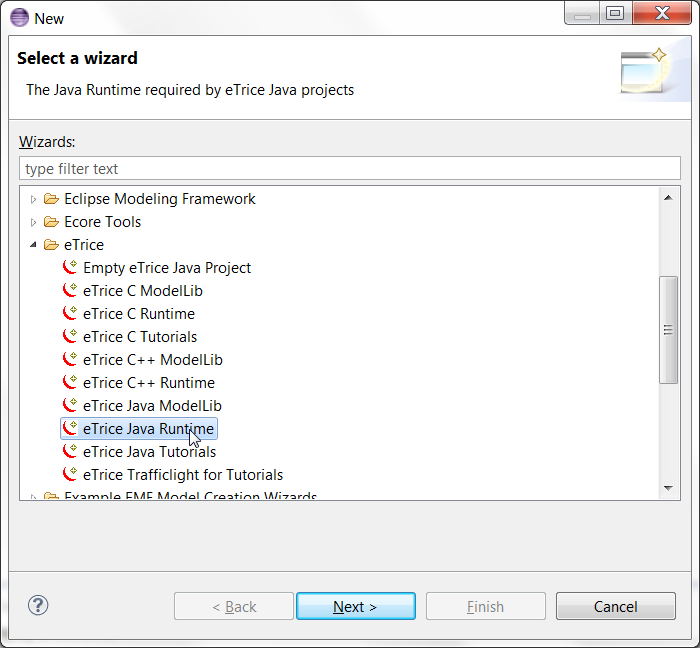
\includegraphics[width=\linewidth]{images/013-SetupWorkspace03.png}
% !images/013-SetupWorkspace03.png!

Do the same steps for \textit{eTrice Java Modellib} and \textit{eTrice Java Tutorials}. To avoid temporary error markers you should keep the proposed order of installation. The resulting workspace should look like this:

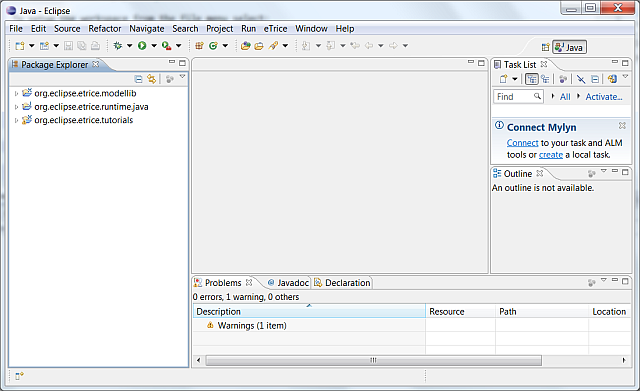
\includegraphics[width=\linewidth]{images/013-SetupWorkspace04.png}
% !images/013-SetupWorkspace04.png!

Now workspace is set up and you can perform the tutorials or start with your work.

The tutorial models are available in the \textit{org.eclipse.etrice.tutorials} project. All tutorials are ready to generate and run without any changes. To start the code generator simply run \textbf{gen\_org.eclipse.etrice.tutorials.launch} as \textbf{gen\_org.eclipse.etrice.tutorials.launch}: 

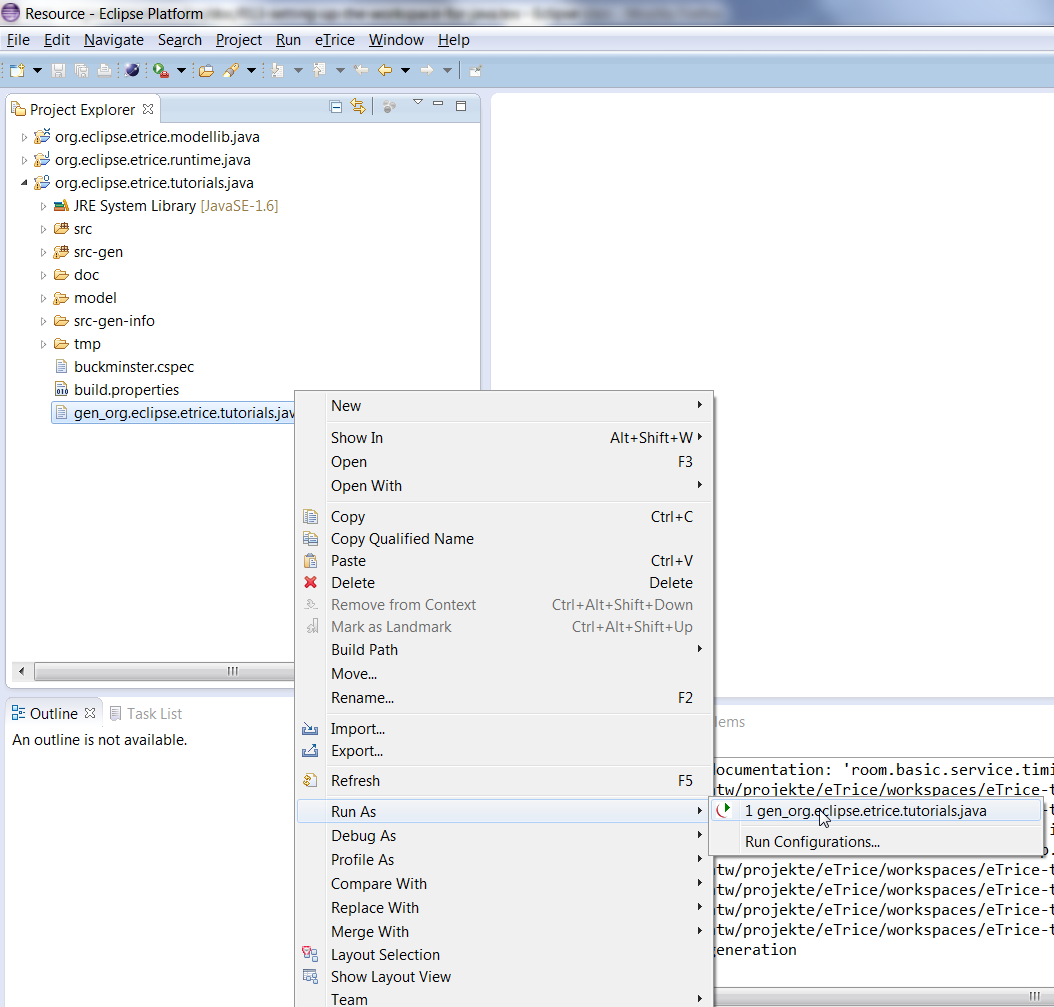
\includegraphics[width=\linewidth]{images/013-SetupWorkspace05.png}
% !images/013-SetupWorkspace05.png!

After generation for each tutorial a java file called \textbf{SubSystem\_ModelnameRunner.java} is generated. To run the model simply run this file as a java application:

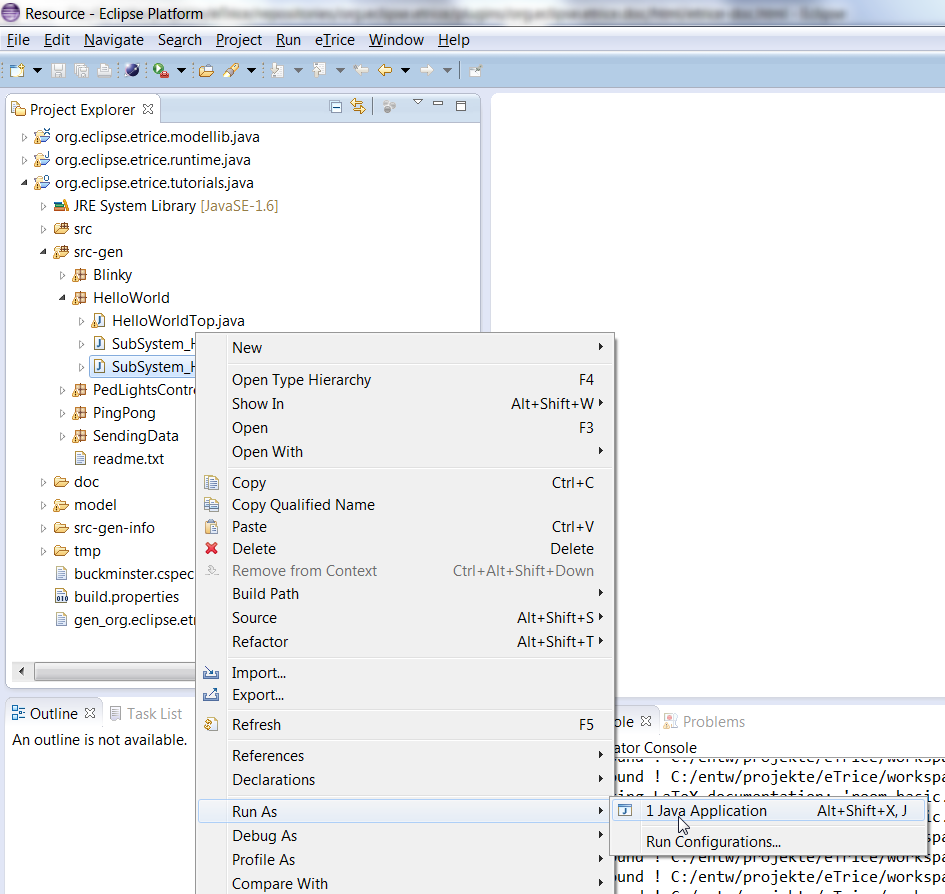
\includegraphics[width=\linewidth]{images/013-SetupWorkspace06.png}
% !images/013-SetupWorkspace06.png!

To stop the application type \textit{quit} in the console window.
 
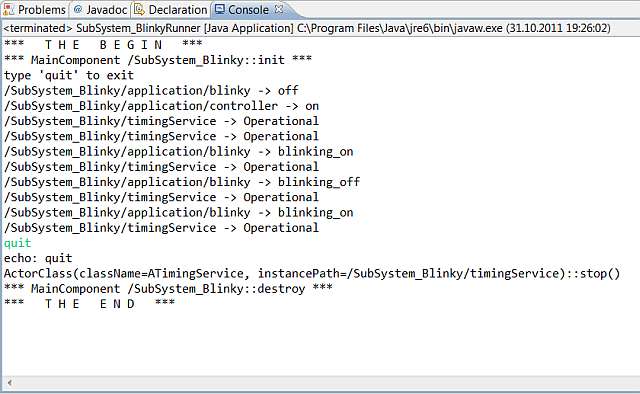
\includegraphics[width=\linewidth]{images/013-SetupWorkspace07.png} 
% !images/013-SetupWorkspace07.png!

Performing the tutorials will setup an dedicated project for each tutorial. Therefore there are some slight changes especially whenever a path must be set (e.g. to the model library) within your own projects. All this is described in the tutorials.
